% Tikz File 'mytikz.tex'
\documentclass{standalone}
\usepackage{tikz}
\usepackage{tikz-qtree}
\usetikzlibrary{calc}

%\usetikzlibrary{...}

\begin{document}

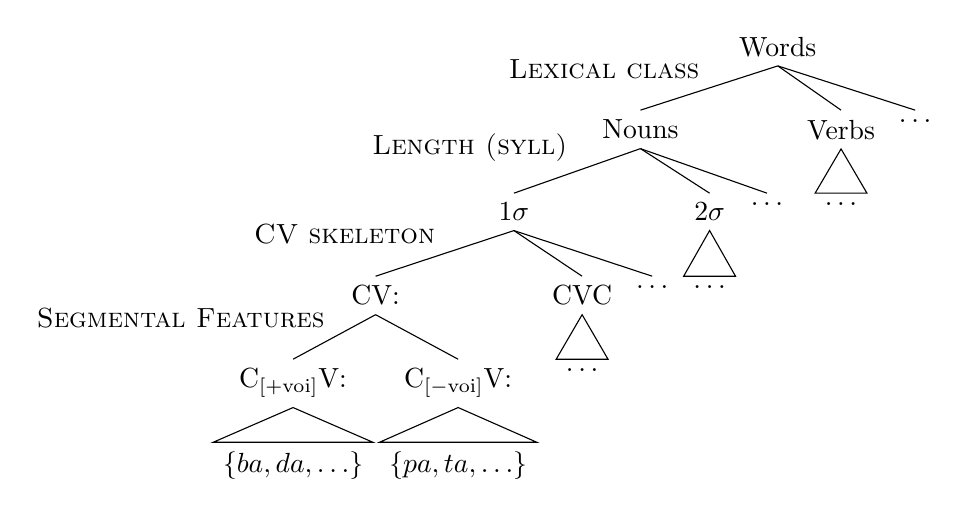
\begin{tikzpicture}%[
  % every tree node/.style={draw,circle},
  % level distance=1.25cm,sibling distance=1cm,
  % edge from parent path={(\tikzparentnode) -- (\tikzchildnode)}]
% \tikzset{edge from parent/.style=
% {draw,
% edge from parent path={(\tikzparentnode.south)
% -- +(0,-8pt)
% -| (\tikzchildnode)}}}
\tikzset{every tree node/.style={align=center,anchor=north}}


\Tree [.Words
           \edge node[auto=right] {\textsc{Lexical class}};
           [.Nouns 
           \edge node[auto=right] {\textsc{Length (syll)}};
                [.1$\sigma$ 
                \edge node[auto=right] {\textsc{CV skeleton}};
                        [.CV: 
                        \edge node[auto=right] {\textsc{Segmental Features}};
                            [.$\mathrm{C_{[+voi]}}$V: \edge[roof]; $\{ba,da,\ldots\}$ ]
                            [.$\mathrm{C_{[-voi]}}$V: \edge[roof]; $\{pa,ta,\ldots\}$ ] ]
                        [.CVC \edge[roof]; {$\ldots$} ]
                        [.$\ldots$ ] ]
                [.2$\sigma$ \edge[roof]; {$\ldots$} ] 
                [.$\ldots$ ] ]
           [.Verbs \edge[roof]; {$\ldots$} ] 
           [.$\ldots$ ] ]
\end{tikzpicture}


\end{document}

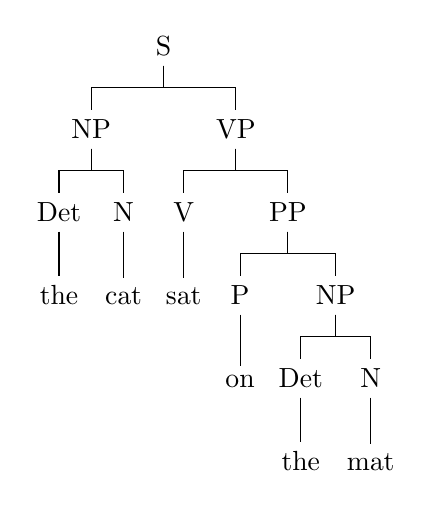
\begin{tikzpicture}
\tikzset{edge from parent/.style=
{draw,
edge from parent path={(\tikzparentnode.south)
-- +(0,-8pt)
-| (\tikzchildnode)}}}
\Tree [.S [.NP [.Det the ] [.N cat ] ]
[.VP [.V sat ]
[.PP [.P on ]
[.NP [.Det the ] [.N mat ] ] ] ] ]
\end{tikzpicture}